\begin{newpage}
  \section{Deliver}
  \label{sec:deliver}

    In diesem Kapitel sollen das Endprodukt und seine Funktionsweise im Gesamtzusammenhang vorgestellt werden. Der erste Abschnitt widmet sich dem generellen Funktionsprinzip und der Kommunikation zwischen Server und Client, bevor im zweiten Abschnitt die einzelnen Funktionen der fertigen Webanwendung beschrieben werden. Im letzten Abschnitt wird schließlich überprüft, inwiefern die Zielsetzungen bezüglich der Performance erreicht werden konnten. 
    
    \subsection{Funktionsprinzip}
\label{sub:funktionsprinzip}
    Für einen Datenaustausch zwischen Server und Client, sind in der fertigen Webanwendung folgende API\footnotemark-Endpunkte vorhanden. 

    \footnotetext{Application Programming Interface}

    \begin{itemize}
      \item \textbf{/daily} stellt die Daten für das Zeitstrahldiagramm bereit und wird beim Start der Anwendung einmalig angefragt. Die Antwort enthält XY-Wertpaare. X stellt dabei die Zeit in Sekunden und Y die zu diesem Zeitwert aktiv werdenden Trips dar.

  \begin{lstlisting}[captionpos=t, caption=Antwort des Servers zur Anfrage \texttt{/daily}, label=lst:daily_response]
  [
    {"x":86340,"y":"6"},
    {"x":86400,"y":"10"}, 
    ...
  ]
  \end{lstlisting}

      \item \textbf{/trips/:from,:to} ermöglicht das Abfragen von Trips, die in einer Zeitspanne \texttt{from - to} aktiv sind. Beim initialen Aufruf der Webanwendung wird dieser Endpunkt als Erstes angefragt, um die aktiven Trips innerhalb einer Stunde zu erhalten. Der gewählte Zeitraum ist in Sekunden anzugeben. 

      Die Antwort des Servers auf einen Endpunkt vom Typ \texttt{/trips/} ist ein Objekt mit der Trip\_Id, dessen Inhalt der \texttt{GeoJSON} Spezifikation nach RFC 7946 folgt:

  \begin{lstlisting}[captionpos=t, caption=Trip Objekt, label=lst:trip_object]
  {
    2498: {  
      "type": "FeatureCollection",
      "features": [
        {
          "type": "Feature",
          "properties": {
            "name": "shape",
            ...
          },
          "geometry": {
            "type": "LineString",
            "coordinates": [[9.4437,48.64482], ...]
          }
        },
        {
          "type": "Feature",
          "properties": {
            "name": "station"
          },
          "geometry": {
            "type": "Point",
            "coordinates": [9.443688, 48.6448]
          }
        },
        ...
      ]
    }
  }
  \end{lstlisting}
    
      Da die Antwort in Listing \ref{lst:trip_object} mittels "`..."' gekürzt ist, sind detailliertere Antworten im \nameref{sec:anhang} unter Listing \ref{lst:geojson_featurecollection}, \ref{lst:shape_feature} und \ref{lst:station_feature} zu finden.

      \item \textbf{/trips/:id} antwortet mit den zur ID gehörenden Trip-Informationen. Dieser Endpunkt ermöglicht es, Informationen für nur einen einzigen Trip zu bekommen. Dies ist vor allem dann hilfreich, wenn der Nutzer ein Vehilce anklickt und Informationen über diesen Trip angezeigt bekommen möchte. Beispiel: \texttt{/trips/51295}

      \item \textbf{/trips/new/:from,:to,:tripIds} stellt die Abfrage für neue Trips zur Verfügung und exkludiert dabei diejenigen Trips, die in \texttt{:tripIds} genannt sind. Damit wird verhindert, dass bereits auf der Karte vorhandene Trips nicht doppelt auftauchen können. Diese Datenbankabfrage wird in einem 30-Sekunden-Intervall vom Client an den Server gesendet, um die neusten Trips zu erhalten. Damit wird die Karte aktuell gehalten. Beispiel: Es ist 10:00 Uhr, hole die in der nächsten Minute aktiv werdenden Trips (Zeitraum 10:00 bis 10:01 Uhr) und schließe die Trips mit der ID \texttt{51295,9212,52} vom Ergebnis aus \texttt{/trips/new/36000,36060,51295,9212,52}.

      \item \textbf{/trips/new/:from,:to} stellt die gleiche Funktionalität wie der vorherige Endpunkt zur Verfügung, mit der Ausnahme, dass keine Trip-ID's übermittelt werden müssen. Dieser Endpunkt ist beispielsweise dafür da, falls die Karte leer ist und noch keine aktiven Trips enthält.

    \end{itemize}

  % subsubsection api_endpunkte (end)

  Das generelle Prinzip der Webanwendung beruht auf einer Client / Server Architektur. Der Nodejs-Server stellt verschiedene Endpunkte mittels Express als ansprechbare Routen dem Client zur Verfügung. 

  \begin{figure}[htbp]
    \begin{center}
      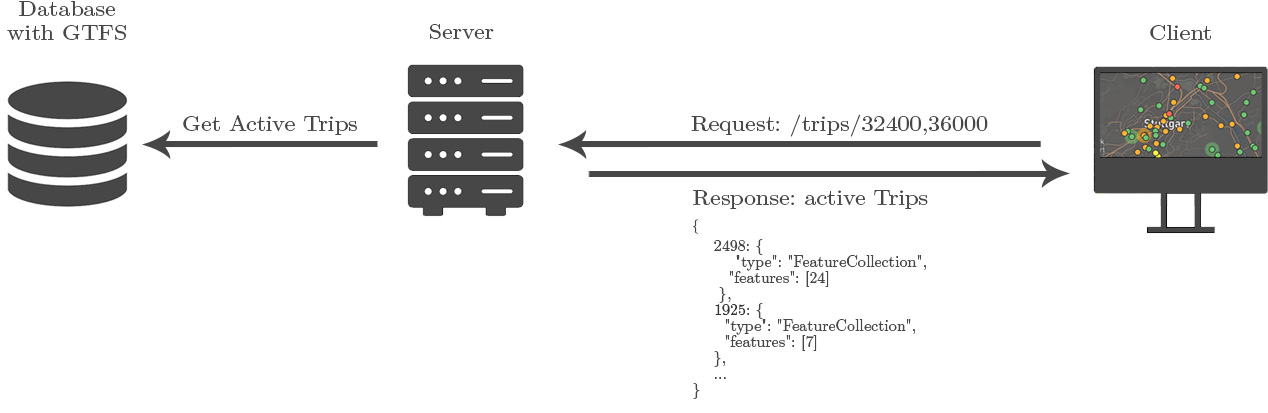
\includegraphics[width=\textwidth]{server_client.jpg}
      \caption{Server / Client Relation}
      \label{fig:server_client}
    \end{center}
  \end{figure}

  Trifft eine valide Anfrage auf den \texttt{/trips/:from,:to} Endpunkt, so wird ein Ablauf nach Abbildung \ref{fig:server_client} angestoßen.
  Die eintreffenden Anfragen werden vom Server entgegengenommen, validiert, verarbeitet und anschließend die entsprechende Antwort zurückgesendet. Die Validierung prüft die vom Client übergebenen Parameter auf ihre Plausibilität. Schlägt diese Prüfung fehl, wird ein Fehler vom Server zurückgegeben und der Server wartet auf eine neue Anfrage. Die wichtigste Routine des Servers stellt die Abfrage von Trips aus der Datenbank dar. Die Datenbank sucht diejenigen Trips heraus, welche in dem benötigten Zeitraum \texttt{from, to} aktiv sind. Dabei wird das Datum und der Wochentag zum Zeitpunkt der Anfrage verwendet. Um die Rechenarbeit im Client zu minimieren, werden alle Daten bei denen dies möglich ist, auf dem Server vorberechnet. Die aus der Datenbank abgefragten Daten durchlaufen folgenden Transformationsprozess:

  \begin{itemize}
    \item \textbf{Daten Mapping:} Die Trips aus der Datenbank werden in das \texttt{GeoJSON}-Format umgewandelt, damit diese im weiteren Programmverlauf einfacher zu verarbeiten sind. Dabei werden die im Kapitel "`\ref{sub:begriffe} \nameref{sub:begriffe}"' festgelegten Regeln beachtet.

    \item \textbf{Zurückgelegte Distanz:} Damit eine Animation der Vehicle stattfinden kann, ist die Berechnung der Distanzen zwischen den einzelnen Stationen nötig. 

    Falls das Feld dist\_traveled\footnotemark in der Datenbank vorhanden ist, kann die zurückgelegte Distanz sehr einfach daraus berechnet werden. Ist dies nicht der Fall, so wird das in Abschnitt \ref{ssub:station_matching} beschriebene Station-Matching durchgeführt, um die Distanzen berechnen zu können.
    \footnotetext{Die zurückgelegte Distanz bis zu einer Station $S$}

    \item \textbf{Feststellen der Richtung:} Für eine Polyline ist es unerheblich, ob die Koordinaten in der Reihenfolge $\{ p_1, p_2, \dotsc, p_n \}$ oder $\{ p_n, \dotsc, p_2, p_1 \}$ angeordnet sind. Damit das Vehicle aber in die richtige Richtung von $A$ nach $B$ fährt, ist es wichtig, dass die Koordinaten der Polyline in aufsteigender Reihenfolge festgelegt werden. Falls dies nicht der Fall ist, werden die Koordinaten in ihrer Reihenfolge umgekehrt.

    \item \textbf{Zeit zwischen Stationen:} In diesem Schritt wird die Fahrzeit (in sec) zwischen den einzelnen Stationen der Trips vorberechnet.

    \item \textbf{Codieren der Polyline:} Hier werden die Koordinaten in einen Polyline-String codiert.

    \item \textbf{Versenden:} Zuletzt wird die Anfrage des Clients vom Server mit einem Response-Paket beantwortet und der Prozess ist damit abgeschlossen bis eine neue Anfrage den Server erreicht.
  \end{itemize}
    
% subsection funktionsprinzip (end)
    \subsection{Funktionen der Webanwendung}
\label{sub:funktionen_der_webanwendung}
  In diesem Abschnitt sollen die verschiedenen UI-Komponenten vorgestellt werden.

  \subsubsection*{Die Karte}
  \label{ssub:die_karte}
    Die Karte (\ref{fig:map}) ist standardmäßig auf den Längengrad 9.244 und Breitengrad 48.757 ausgerichtet. Damit findet sich der Anwender beim Aufrufen der Applikation gleich an der richtigen Stelle wieder. Die Karte verwendet eine abgeänderte Version des Kartenstils \texttt{Mapbox-Dark}. Dabei wurden Parks, Grünflächen und Wasser subtil eingefärbt und die Routen des GTFS-Feeds mit einem leichten Orange hervorgehoben.

    \begin{figure}[htbp]
      \begin{center}
        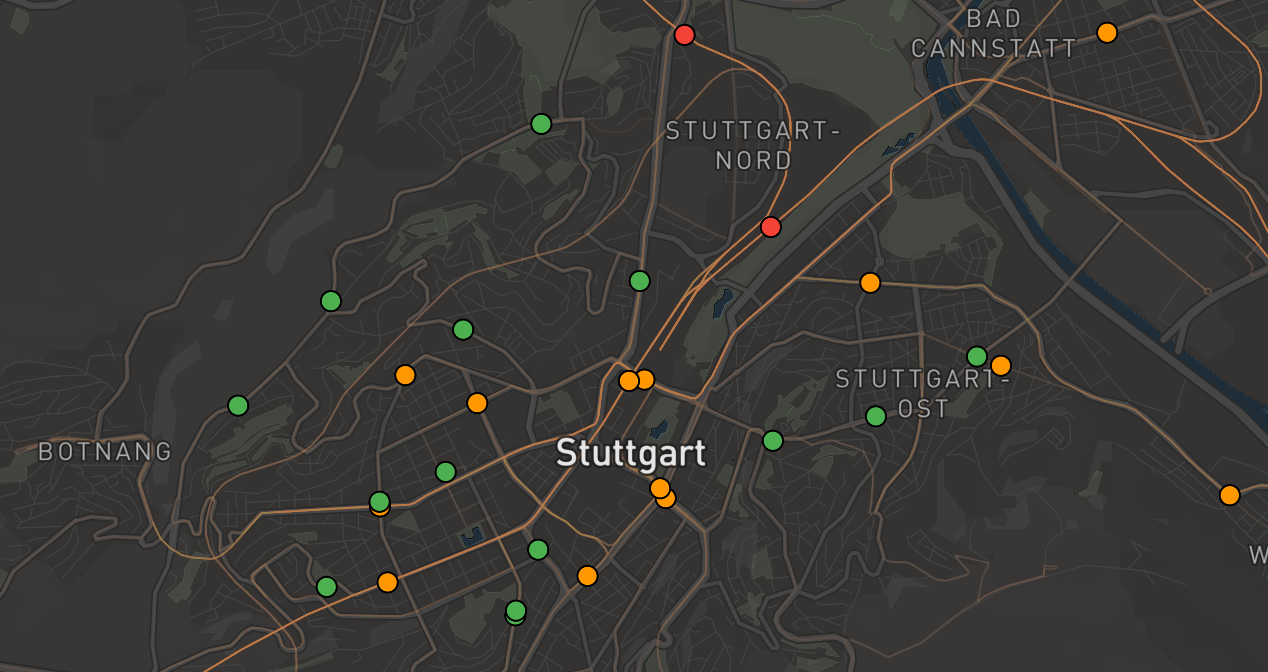
\includegraphics[width=0.6\textwidth]{map}
        \caption{Die Karte mit angepasstem Style: Mapbox-Dark}
        \label{fig:map}
      \end{center}
    \end{figure}
    
  % subsubsection die_karte (end)

  \subsubsection*{Vehicle}
  \label{ssub:vehicle_auf_karte}
    Die Vehicle sind auf der Karte als Kreis dargestellt. Die verwendete Farbe orientiert sich dabei an den offiziellen Farben des jeweiligen Verkehrsunternehmens. Zum Beispiel sind Interrail Züge im Rot der Deutschen Bahn dargestellt und die U- und S-Bahnen im Orange des Stuttgart-VVS.\\

    Vehicle werden auf der Karte animiert, wenn sie aktiv sind. Abbildung \ref{fig:vehicle_states} zeigt die zwei verschiedenen Animationen, die ein Vehicle beim Start und Beenden des Trips annehmen kann. Wird ein Trip aktiv, so wird das dazugehörende Vehicle mit vergrößertem Radius auf die Karte platziert. Danach wird der Radius des Vehicles in kurzer Zeit verringert, bis er der Radiusgröße der anderen Vehicle entspricht.

    \begin{figure}[htbp]
      \centering
      \subfloat[Vehicle beginnt seinen Trip und wird aktiv]{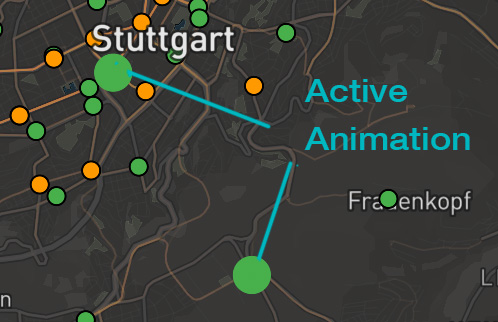
\includegraphics[width=0.34\textwidth]{vehicle_active.jpg}\label{fig:vehicle_active}}
      \hfill
      \subfloat[Vehicle beendet seinen Trip innerhalb von 30 Sekunden und wird inaktiv]{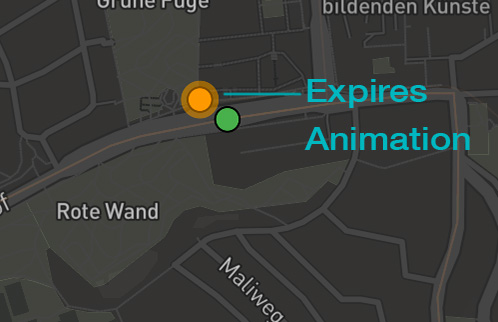
\includegraphics[width=0.34\textwidth]{vehicle_expires.jpg}\label{fig:vehicle_expires}}
      \caption{Vehicle Status Anzeige}
      \label{fig:vehicle_states}
    \end{figure}

    
    Ist ein Vehicle dabei, seinen Trip innerhalb von 30 Sekunden zu beenden, so wird ein leicht transparentes Pulsieren angezeigt. Nachdem das Vehicle den Trip beendet hat, wird es von der Karte genommen und verschwindet. Technisch betrachtet, werden erst alle Referenzen auf das Vehicle beseitigt und anschließend das Vehicle-Objekt gelöscht.
    
  % subsubsection vehicle (end)

  \subsubsection*{Zeitstrahl}
  \label{ssub:zeitstrahl}
    Die Webanwendung besitzt einen interaktiven Zeitstrahl am unteren Bildrand. Wie in Abbildung \ref{fig:timeline} zu sehen, besteht der Zeitstrahl aus mehreren Einzelteilen. 

    \begin{figure}[htbp]
      \begin{center}
        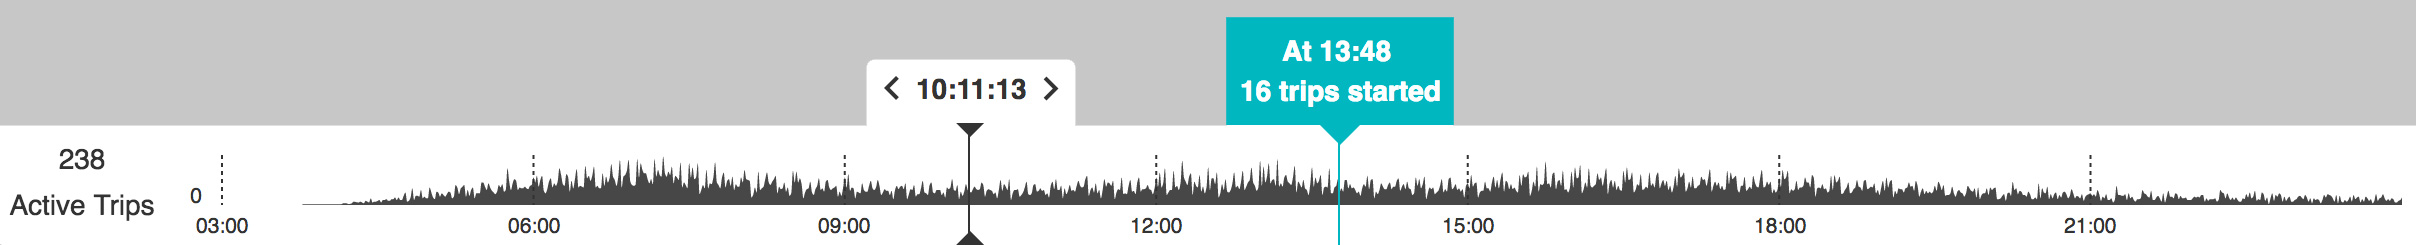
\includegraphics[width=\textwidth]{timeline}
        \caption{Zeitstrahl Komponente}
        \label{fig:timeline}
      \end{center}
    \end{figure}

    Links unten ist die Anzahl an momentan aktiven Trips zu sehen. Diese Anzahl korreliert mit den Vehicles auf der Karte. Die Anzeige wird immer aktuell gehalten und steigt, falls neue Trips aktiv werden, oder fällt wenn ein Trip beendet ist. Der Zeitstrahl selbst zeigt die Anzahl an aktiv werdenden Trips pro Minute an. Bewegt der Anwender die Maus darüber, so bekommt er die genaue Trip-Anzahl zu einer Uhrzeit als Tooltip angezeigt. Ebenfalls ist es möglich, die Animation zu einem beliebigen Zeitpunkt anzuzeigen. Dafür kann der Anwender einfach auf die gewünschte Zeitmarke im Zeitstrahl klicken und die Animation aktualisiert sich. Damit lässt sich die Karte zu unterschiedlichen Tageszeiten untersuchen. Zuletzt ist auch die gewählte Uhrzeit auf dem Zeitstrahl zu sehen. Diese zeigt dem Anwender, welcher Zeitpunkt momentan auf der Karte angezeigt wird.
    
  % subsubsection zeitstrahl (end)

  \subsubsection*{Filter}
  \label{ssub:filter}
    Über ein ausklappbares Menü lassen sich verschiedene Filter auswählen. Dadurch kann der Anwender zum Beispiel alle Vehicle eines Typs oder einer Linie abrufen. Auch Kombinationen der \texttt{Filter Vehicles} und \texttt{Filter Lines} sind möglich.

    Damit der Anwender die Relation zwischen Filter und Vehicles auf der Karte versteht, sind die Farben einheitlich gestaltet. Nachdem ein Filter ausgewählt ist, kann das Menü entweder wieder zugeklappt oder der Filter abgewählt werden.

    \begin{figure}[htbp]
      \begin{center}
        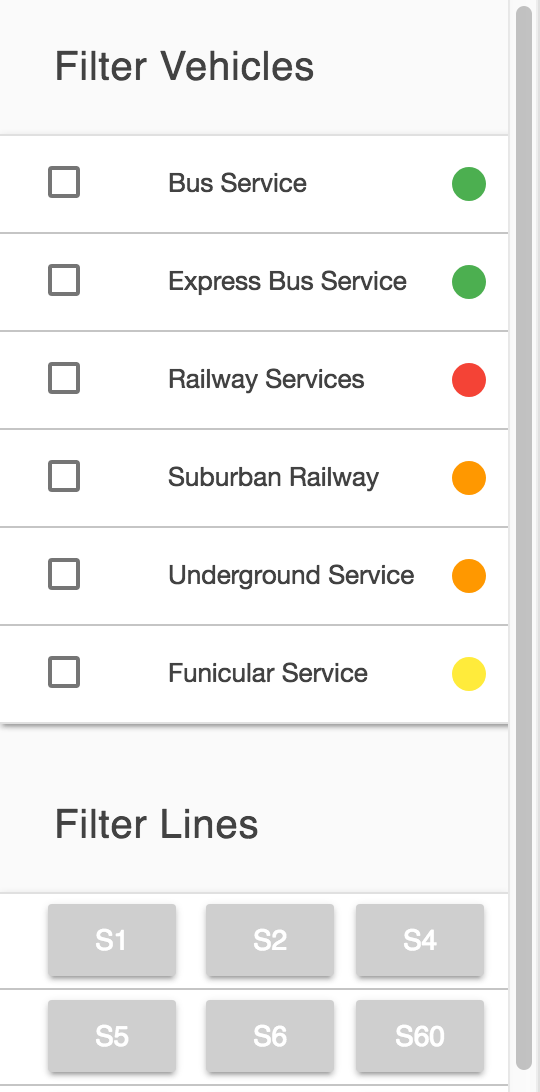
\includegraphics[width=0.2\textwidth]{filter}
        \caption{Filter Funktion}
        \label{fig:filter}
      \end{center}
    \end{figure}
    
  % subsubsection filter (end)

  \subsubsection*{Anzeigen von Trip Informationen}
  \label{ssub:anzeigen_von_trip_informationen}
    Wenn der Anwender ein Vehicle in der Karte durch Klicken auswählt, öffnet sich ein Fenster, welches Informationen für diesen Trip anzeigt (Abbildung \ref{fig:trip_information}. Neben dem Namen der Route lässt sich im Kreis (hier in Rot) die Routennummer ablesen. Im unteren Bereich sind die Fahrplaninformationen für den Trip gelistet. Neben dem Namen der Station ist auch die Abfahrtzeit des Vehicles gelistet. Die bereits besuchten Stationen werden in einem Grauton dargestellt, um sie als inaktiv zu markieren.

    \begin{figure}[htbp]
      \begin{center}
        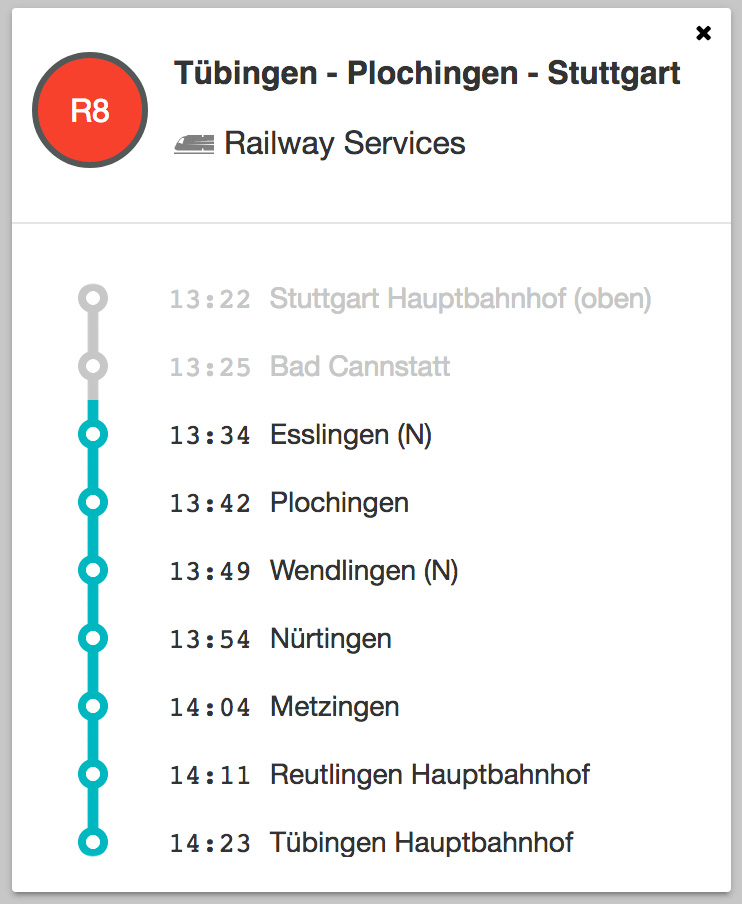
\includegraphics[width=0.3\textwidth]{trip_information}
        \caption{Anzeigen von Trip Informationen}
        \label{fig:trip_information}
      \end{center}
    \end{figure}
    
  % subsubsection anzeigen_von_trip_informationen (end)

  \subsubsection*{Wechseln der Kartendarstellung}
  \label{ssub:style_auswahl}
    Über das \texttt{Switch Style} Element {\Large \inlinegraphics{switch_styles_symbol}} hat der Anwender die Möglichkeit, zwischen verschiedenen Darstellungsarten der Karte zu wechseln. Auch die Polylines der Routen lassen sich zusätzlich über das Anwählen von \texttt{Shape} ein- oder ausblenden. Standardmäßig ist \texttt{Dark} ausgewählt.

    \begin{figure}[htbp]
      \begin{center}
        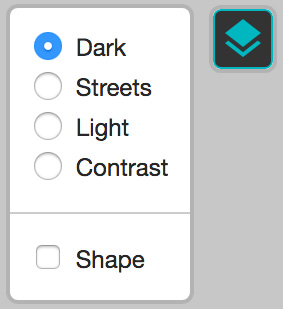
\includegraphics[width=0.14\textwidth]{switch_styles}
        \caption{Wechseln zwischen verschiedenen Kartendarstellung}
        \label{fig:switch_styles}
      \end{center}
    \end{figure}
    
  % subsubsection style_auswahl (end)

  \subsubsection*{Wegfindung}
  \label{ssub:wegfindung}
    Durch Klicken des \texttt{Line Finder} Buttons {\Large \inlinegraphics{line_finder_symbol}} lässt sich auf der Karte eine Route finden, die zwei Stationen $A, B$ verbindet. Dafür setzt der Anwender zwei Pins auf die Karte. Danach sucht ein Algorithmus diejenige Route aus, die am besten diese Stationen verbindet. Das Ergebnis sieht dann wie folgt aus:

    \begin{figure}[htbp]
      \begin{center}
        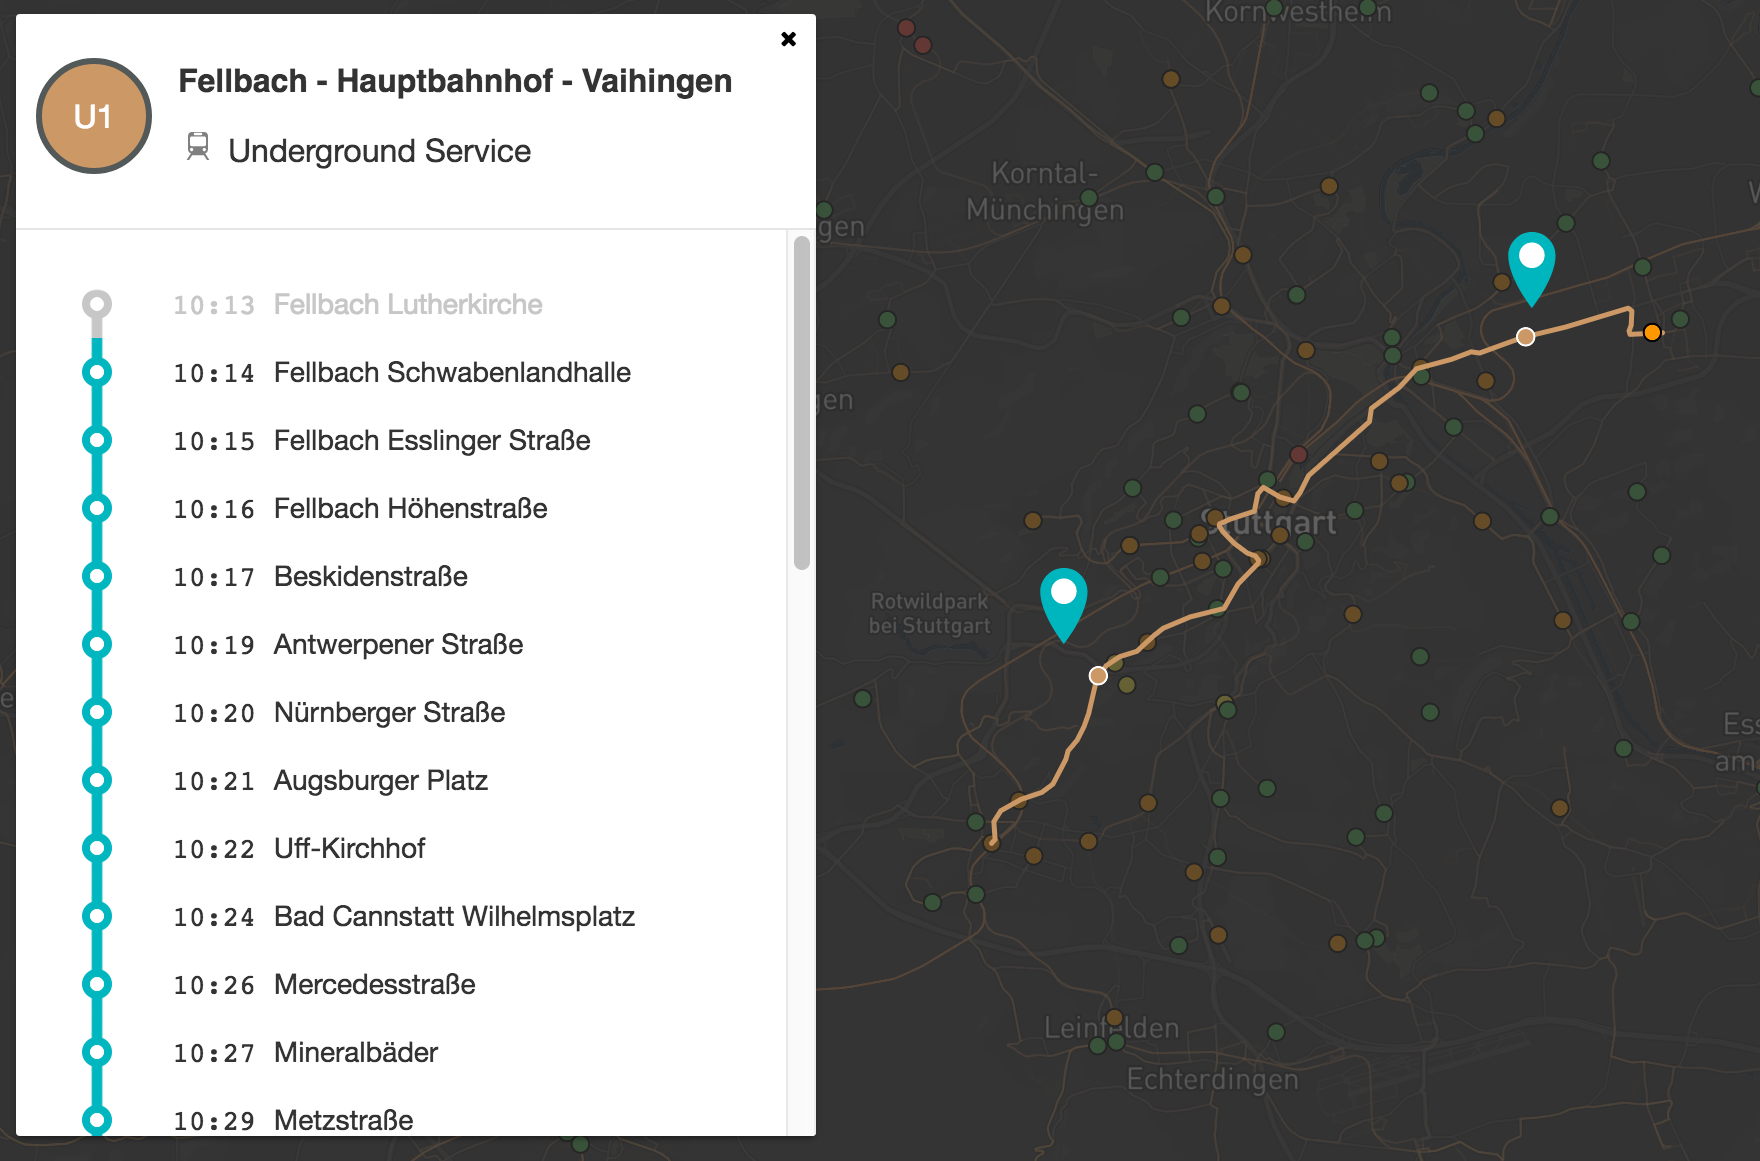
\includegraphics[width=0.6\textwidth]{line_finder}
        \caption{Linien Finder}
        \label{fig:line_finder}
      \end{center}
    \end{figure}

    Diese Funktion vereint Visualisierung und Wegfindung in einer Applikation. Während wir von anderen Applikationen gewohnt sind, eine Wegfindung ausschließlich über verschiedene Formularfelder (Von..., Nach..., Datum, Uhrzeit) anzufragen, könnte es für städtische oder regionale Wegfindung auch eine visuelle Lösung geben. Der Vorteil liegt dabei, dass kein Kontextwechsel nötig ist. Die Orientierung, Wegfindung und Fahrplaninformationen ließen sich alle in einer Ansicht vereinen. Ein weiteres Merkmal dieses visuellen Ansatzes ist die Möglichkeit, eine Route zu finden, ohne dass die Namen der Haltestellen bekannt sein müssen. Das auf der Karte dargestellte Ergebnis zeigt dem Nutzer auch sofort, wo sich das zur Route gehörende Vehicle momentan (oder zu einem bestimmten Zeitpunkt) befinden müsste. Damit könnte der Anwender auch gleich entscheiden, ob er dieses Vehicle noch erreichen würde oder nicht. Insbesondere an dieser Stelle wären GTFS-Realtime-Informationen von Nutzen, mit welchen beispielsweise Verspätungen mitangezeigt werden können.\\

    Von allen implementierten Komponenten bietet der Linien Finder das größte Potential für verschiedenste Weiterentwicklungen. Angefangen von der Implementierung von Echtzeitinformationen, über eine integrierte Anwender-Navigation (zum Beispiel könnte man den Anwender zu einer Station navigieren), bis zum Anbieten von Verbindungsanschlüssen bestünden Entwicklungsmöglichkeiten. Darüber hinaus kann der Algorithmus zur Auswahl der empfohlenen Route noch sehr viel weiter verbessert werden. Momentan fließt vor allem die mittlere Distanz zwischen gesetztem Pin und nächster Station in die Entscheidung ein. Weitere Faktoren könnten aber noch berücksichtigt werden. Beispielsweise der Typ des Vehicles (U-Bahn bevorzugt gegenüber Bus), Frequenz der Route, Wartezeit auf das Vehicle, Preis, Reisezeit oder gar das momentane Verkehrsaufkommen.
    
  % subsubsection linien_finder (end)
    
    % * Timeline Component (Time jump + Trip counter, Trips that get active)
    % * Vehicles, Vehicle States (active, inactive)
    % * Filtering mechanism (Lines / Type)
    % * Layer switcher
    % * Route finder
    % * Bezier Easing 
    
% subsection funktionen_der_webanwendung (end)
    \subsection{Ergebnisse}
\label{sub:ergebnisse}
  Durch die Anwendung war es möglich, die Daten über einen ganzen Tag hinweg aufzuzeichnen und in einem Diagramm darzustellen. Dabei bilden die Daten die Aktivität des öffentlichen Nahverkehrs in Stuttgart an einem Montag den 28.08.2017 zwischen 3.00 und 24.00 Uhr ab. Abbildung \ref{fig:activeTrips} zeigt, dass nach einem rapiden Anstieg in der Morgenzeit um 07:04 Uhr ein Höhepunkt mit 799 aktiven Trips erreicht wird.

  \begin{figure}[ht]
    \begin{center}
      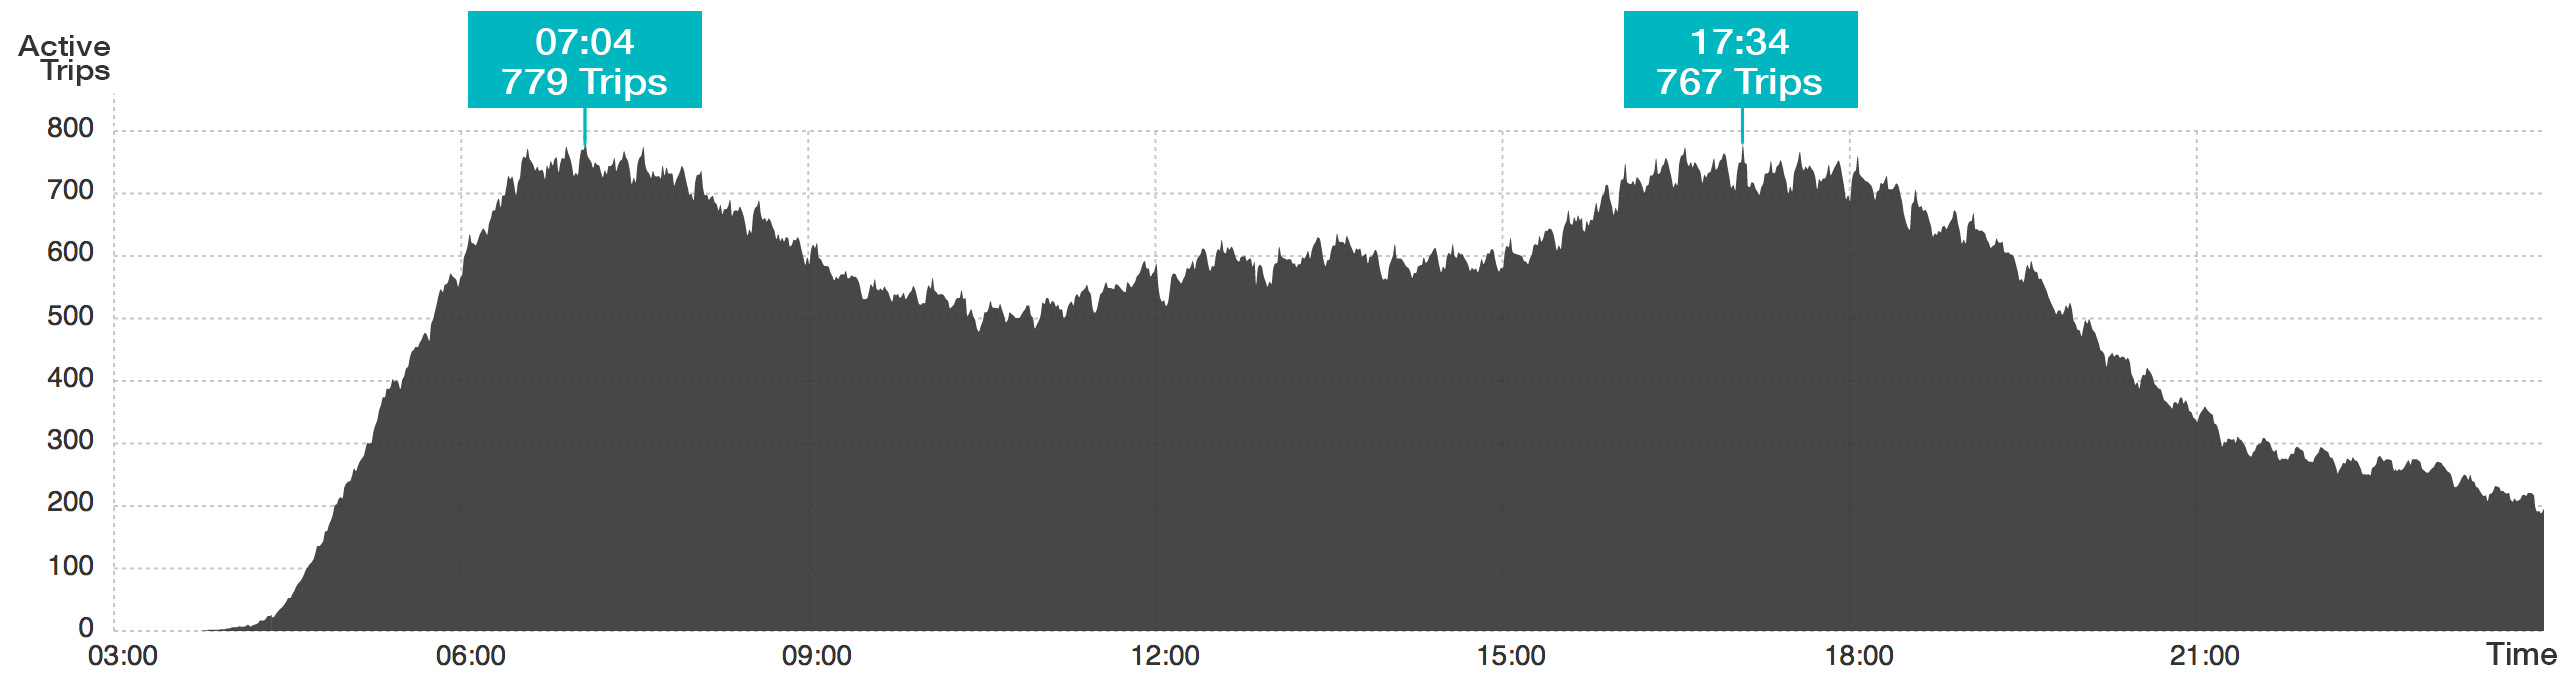
\includegraphics[width=\textwidth]{activeTrips.jpg}
      \caption{Anzahl an aktiven Trips zwischen 3.00 und 24.00 Uhr am 02.08.2017}
      \label{fig:activeTrips}
    \end{center}
  \end{figure}

  Anschließend flacht Mittags die Aktivität leicht ab, um dann zur Rush Hour am Abend wieder auf 767 gleichzeitig aktive Trips anzusteigen. Letztlich flacht die Anzahl immer weiter ab, um am nächsten Tag gegen 3 Uhr wieder anzusteigen und der Kreislauf beginnt von neuem. Insgesamt wurden an diesem Tag knapp 19650 Trips absolviert. Das Maximum betrug dabei $27 \frac{Trips}{Minute}$ wohingegen das Minimum bei $0 \frac{Trips}{Minute}$ lag. Im Schnitt starten 9 Vehicles pro Minute ihre Fahrt. Für eine interaktive Karte bedeutet dies, dass je nach Tag zwischen 0 und 1000 Trips aktiv sein können. Dies entspricht dann auch der Anzahl an Vehicle, die sich auf der Karte bewegen und animiert werden müssen. Sowohl durch die verschiedenen Frontend-Optimierungen aus Kapitel \ref{ssub:verbesserung_der_client_performance}, als auch durch die Anpassung von verschiedenen Bibliotheksfunktionen, konnte durchgängig ein Rendering mit 60 FPS im Frontend erreicht werden. Damit wurde dieses gesetzte Teilziel erreicht.\\

  Für die Ergebnisse der Evaluierung des Gesamtsystems wurden die Verarbeitungszeit des Servers, als auch die Antwortzeit der Datenbank in einem Zusammenhang betrachtet. Folgende Metriken lassen sich für dieses Gesamtsystem feststellen:

  \begin{longtable}{|>{\raggedright \arraybackslash}p{4.5cm}|>{\raggedright \arraybackslash}p{1.2cm}|>{\raggedright \arraybackslash}p{1.2cm}|>{\raggedright \arraybackslash}p{1.2cm}|>{\raggedright \arraybackslash}p{1.2cm}|>{\raggedright \arraybackslash}p{1.2cm}|>{\raggedright \arraybackslash}p{1.2cm}|}
  \caption{Backend Evaluation}\label{tbl:backend_evaluation}\\
    \hline
    Anz. Trips & 20 & 100 & 500 & 1000 & 5000 & 10000\\
    \hline
    Query Zeit (ms)        & 25 & 88 & 124 & 200 & 855 & 1631 \\
    Verarbeitungszeit (ms) & 2 & 27 & 40 & 142 & 226 & 435 \\
    Summe (ms)             & 27 & 115 & 164 & 342 & 1081 & 2066 \\
    \hline
  \end{longtable}

  In Tabelle \ref{tbl:backend_evaluation} sind die Datenwerte für verschiedene Abfragen aufgelistet. Die Werte ergeben sich aus dem Mittelwert der Laufzeit in 10 Durchläufen.\\

  Aus dieser Aussage plus den gemessenen Werten lässt sich folgende Schlussfolgerung ziehen: Bei einer Anzahl zwischen 20 und 100 Trips reagiert der Server innerhalb von 25 bis $120ms$. Da die meisten Trips in diese Spanne fallen, ist dieses Ergebnis am bedeutendsten. 

  Im Bereich von 100 bis 500 Trips ist eine Antwortzeit von 115 bis $164ms$ immer noch sehr gut. Diese Anzahl an Trips ist dann relevant, wenn die Applikation das erste Mal aufgerufen wird und die Karte noch leer ist. In diesem Fall kann es sein, dass der Server (je nach Datum und Uhrzeit) zwischen 200 - 500 Trips verarbeiten muss. Aber selbst Abfragen von bis zu 10.000 Trips, was ungefähr einer Zeitspanne von einem Tag gleich kommt, sind immer noch innerhalb von 2 Sekunden verarbeitet.\\

  Abschließend kann gesagt werden, dass in dieser Arbeit ein performantes Backendsystem für eine Web Applikation entwickelt worden ist, welches Serveranfragen effizient be- und verarbeiten kann.
  
% subsection ergebnisse (end)
    
  % section deliver (end)
\end{newpage}